\documentclass[11pt,a4paper]{article}

\usepackage[utf8]{inputenc}
\usepackage[T1]{fontenc}
\usepackage{lmodern}
\usepackage[french]{babel}
\usepackage[margin=2.4cm]{geometry}
\usepackage{microtype}
\usepackage{booktabs}
\usepackage{array}
\usepackage[table]{xcolor}
\usepackage{amsmath}
\usepackage{amssymb}
\usepackage{mathtools}
\usepackage{enumitem}
\usepackage[most]{tcolorbox}
\usepackage{tabularx}
\usepackage{graphicx}
\usepackage{caption}
\usepackage{titlesec}
\usepackage[section]{placeins}
\usepackage{hyperref}

\definecolor{navy}{HTML}{1F3864}
\definecolor{bluemid}{HTML}{2E5496}
\definecolor{lightblue}{HTML}{D6E0F0}
\definecolor{accent}{HTML}{C0491F}

\hypersetup{colorlinks=true, linkcolor=bluemid, urlcolor=bluemid,
  pdftitle={Calibrer le facteur systemique - ancienne et nouvelle methode},
  pdfauthor={Kelian Kaddouri}}

\newtcolorbox{cle}[1][]{colback=lightblue!40,colframe=navy,boxrule=0.6pt,
  arc=2pt,left=8pt,right=8pt,top=6pt,bottom=6pt,before skip=9pt,after skip=9pt,#1}
\newtcolorbox{attention}[1][]{colback=accent!8,colframe=accent,boxrule=0.6pt,
  arc=2pt,left=8pt,right=8pt,top=6pt,bottom=6pt,before skip=9pt,after skip=9pt,#1}

\titleformat{\section}{\normalfont\large\bfseries\color{navy}}{\thesection}{0.6em}{}
\titlespacing*{\section}{0pt}{1.9ex plus .3ex minus .2ex}{1.0ex plus .2ex}
\titleformat{\subsection}{\normalfont\normalsize\bfseries\color{bluemid}}{\thesubsection}{0.6em}{}
\captionsetup{font=small,labelfont={bf,color=navy},labelsep=period,skip=6pt}
\renewcommand{\topfraction}{0.92}
\renewcommand{\bottomfraction}{0.85}
\renewcommand{\textfraction}{0.07}

\newcommand{\Y}{Y}
\newcommand{\eps}{\varepsilon}

\title{\vspace{-1.2cm}\color{navy}\bfseries Calibrer le facteur systémique des piliers DORA\\[2pt]
  \large En quoi la nouvelle méthode diffère de l'ancienne}
\author{Kélian Kaddouri}
\date{\today}

\begin{document}
\maketitle
\vspace{-0.6cm}

\begin{cle}
\textbf{Deux résultats, dans cet ordre.} \emph{(1)}~L'estimateur de la contagion~$W$ que la
note utilisait depuis le début comportait une \textbf{erreur d'indexation} : les indicatrices
de période n'absorbaient rien. Elle est corrigée, et sa signature est instructive. \emph{(2)}~La
généralisation~A du modèle (un facteur systémique $\Y_j$ \emph{par pilier}, des charges $s_j$,
une matrice de dépendances croisées $\Sigma_Y$) était \textbf{posée sans protocole
d'estimation}. Elle en a désormais deux, dont l'un ne requiert
\textbf{aucune donnée individuelle}. Conséquence pour le mémoire : le verrou empirique est
\textbf{plus étroit} que ne l'annonçait le chapitre de faisabilité.
\end{cle}

\section{Un bug d'indexation, et sa signature}

\subsection{L'erreur}

Le probit du script \texttt{03} régresse l'incident du pilier~$j$ à la période~$t$ sur les
incidents \emph{retardés} des quatre autres piliers, avec des \textbf{effets fixes de
période} destinés à absorber le systémique $s_j \Y_{j,t}$. Le panel est aplati par
\texttt{reshape(-1)} sur un tableau de forme $(N, T-1)$, donc \textbf{ligne par ligne} :
l'observation~$m$ est l'entité $m \,//\, (T-1)$ à la période $m \bmod (T-1)$.

\begin{verbatim}
    per_idx = np.repeat(np.arange(T - 1), N)     # ANCIEN -- faux
    per_idx = np.tile(np.arange(T - 1), N)       # NOUVEAU -- correct
\end{verbatim}

\noindent
Avec \texttt{repeat}, chaque indicatrice était collée à un bloc d'entités, pas à une période.
Les effets fixes n'absorbaient \textbf{rien}.

\subsection{Pourquoi la faute était invisible}

Si $s_j \Y_{j,t}$ reste dans le terme d'erreur, la variance de celui-ci passe de $1$ à
$1 + s_j^2$. Or un probit n'identifie ses coefficients qu'\emph{à l'échelle de l'erreur près}.
Tous les coefficients sont donc \textbf{atténués} du facteur
\begin{equation}
\frac{1}{\sqrt{1+s_j^{2}}} \;=\; \frac{1}{\sqrt{1+0{,}5^{2}}} \;=\; 0{,}894 .
\end{equation}
La pente estimée valait $0{,}92$. Elle \emph{devait} valoir~$1$. Un écart de $8\,\%$ vers le
bas, sur un estimateur bruité : rigoureusement indiscernable d'un estimateur qui fonctionne.
Le rapport observé après correction, $0{,}92 / 1{,}08 = 0{,}85$, est bien du bon ordre de
grandeur que prédit l'atténuation.

\begin{attention}
\textbf{Un estimateur qui rend le chiffre attendu n'est pas pour autant correct.} Le bug ne
produisait pas d'aberration : il produisait un résultat \emph{plausible}. Il n'a été démasqué
que par une tâche \emph{ultérieure}, l'extraction de $\Y_j$ à partir de ces mêmes effets
fixes, qui rendait $\mathrm{corr}(\hat{\Y}, \Y) = 0{,}05$ et $\hat{s}_j \approx 0{,}04$ pour
tous les piliers. C'est la tentative de faire la chose suivante qui a révélé l'erreur dans la
chose précédente.
\end{attention}

\subsection{Ce que la correction déplace}

\begin{table}[h]
\centering
\small
\caption{Script \texttt{03}, avant et après correction de l'indexation. Panel simulé
$N = 800$ entités $\times$ $T = 60$ périodes $\times$ $5$ piliers.}
\begin{tabular}{lcc}
\toprule
\textbf{Diagnostic} & \textbf{Ancien} (\texttt{repeat}) & \textbf{Nouveau} (\texttt{tile}) \\
\midrule
Corrélation $\hat W$ vs $W$ (probit)      & $0{,}83$  & $\mathbf{0{,}92}$ \\
Pente $\hat W$ sur $W$ (probit)           & $0{,}92$  & $\mathbf{1{,}08}$ \\
Pente $\hat W$ sur $W$ (logit)            & $1{,}83$  & $2{,}11$ \\
Sens de l'asymétrie correctement retrouvé & --        & $\mathbf{100\,\%}$ \\
\midrule
Corrélation à $N = 400$                   & $0{,}43$  & $\mathbf{0{,}90}$ \\
\midrule
Asymétrie, panel réel                     & $1{,}15$  & $1{,}57$ \\
Asymétrie, après permutation (placebo)    & $0{,}39$  & $0{,}38$ \\
Corrélation $W$ avant / $W$ temps inversé & $-0{,}40$ & $-0{,}70$ \\
\bottomrule
\end{tabular}
\end{table}

\noindent
La pente passe au-dessus de~$1$, comme le veut la théorie du probit : $W$ est retrouvée
\textbf{dans ses propres unités}, ce qui confirme au passage que l'estimateur naturel est un
probit et non un logit (dont la pente $2{,}11$ signale des magnitudes exprimées en unités
logistiques). Et la puissance du protocole était très sous-estimée : $N = 400$ entités
suffisent désormais, contre plusieurs milliers apparemment requis auparavant.

\section{La nouvelle méthode : calibrer $\Y_j$, $s_j$ et $\Sigma_Y$}

\subsection{Ce que l'ancienne méthode ne faisait pas}

La note posait la généralisation~A,
\begin{equation}
X_{i,j,t} \;=\; \underbrace{\text{base}_j}_{\text{niveau}}
\;+\; \underbrace{\textstyle\sum_{k \neq j} W_{jk}\, D_{i,k,t-1}}_{\text{contagion dirigée}}
\;+\; \underbrace{s_j\, \Y_{j,t}}_{\text{systémique, propre au pilier}}
\;+\; \eps_{i,j,t}, \qquad \Y_t \sim \mathcal{N}(0, \Sigma_Y)
\end{equation}
puis s'arrêtait là. \textbf{Aucun protocole n'était proposé pour $\Y_j$, $s_j$, $\Sigma_Y$.}
Le seul objet calibré était $W$. C'est le trou qui vient d'être comblé, par deux routes
indépendantes.

\subsection{Route A : lire les effets fixes qu'on avait déjà}

Une fois l'indexation corrigée, les effets fixes de période du probit valent \emph{exactement}
$\varphi_{j,t} = \text{base}_j + s_j \Y_{j,t}$. Il n'y avait rien à estimer de plus : il
suffisait de les \emph{lire}.
\begin{equation}
\text{base}_j = \overline{\varphi_{j,\cdot}}, \qquad
\hat{s}_j = \mathrm{sd}_t(\varphi_{j,t}), \qquad
\hat{\Y}_{j,t} = \frac{\varphi_{j,t} - \text{base}_j}{\hat{s}_j}, \qquad
\hat{\Sigma}_Y = \mathrm{corr}(\varphi) .
\end{equation}
La dernière égalité tient parce qu'une corrélation est \textbf{insensible à l'échelle} $s_j$.
Le prix à payer : la route~A exige un panel \emph{entité $\times$ pilier $\times$ période}.

\subsection{Route B : la distance de Frobenius, sur données agrégées}

Transposition directe de la méthode de Pineau et Zuñiga (2023, éq.~5), qui extraient leur
facteur latent en minimisant la distance de Frobenius entre matrices de transition observées et
engendrées. Ici, pour chaque période~$t$, on n'observe que des \textbf{comptages agrégés} :
\begin{align}
\Pi^{\text{obs}}_{jk} &= \mathbb{P}(\text{incident en } j \text{ à } t
   \;\wedge\; \text{incident en } k \text{ à } t-1) && (25 \text{ moments}) \\
m^{\text{obs}}_{j}   &= \mathbb{P}(\text{incident en } j \text{ à } t)
   && (5 \text{ moments})
\end{align}
et l'on résout, à $W$ et base connues, un problème de $30$~équations pour $5$~inconnues
$u_{j,t} = s_j \Y_{j,t}$ :
\begin{equation}
\hat{u}_t \;=\; \arg\min_{u \in \mathbb{R}^5}
  \Bigl\lVert \Pi^{\text{obs}} - \Pi^{\text{mod}}(u) \Bigr\rVert_F^2
  \;+\; \omega^2 \bigl\lVert m^{\text{obs}} - m^{\text{mod}}(u) \bigr\rVert^2 ,
  \qquad \omega = 3 .
\end{equation}
Les moments du modèle s'obtiennent en énumérant les $2^5 = 32$ configurations possibles
d'incidents à $t-1$, sous indépendance des piliers à la période retardée.

\begin{attention}
\textbf{Les moments marginaux sont indispensables, et c'est un piège coûteux.} Ma première
version n'utilisait que les $25$ co-incidences. Elle rendait $\mathrm{corr}(\hat{\Y}, \Y) =
0{,}835$ et sur-estimait $\hat{s}_j$ du \emph{double}. J'ai d'abord cru au bruit
d'échantillonnage : le fractionnement d'échantillon ne corrigeait rien ($0{,}697$ contre
$0{,}694$), donc le biais était \textbf{commun aux deux moitiés} : il était structurel, pas
aléatoire. Diagnostic : le résidu corrélait à $+0{,}36$ avec le systémique \emph{retardé}
$\Y_{t-1}$, parce que les co-incidences ne portent que sur les $\approx 6\,\%$ d'entités ayant
déjà subi un incident en $t-1$. $u_j$ y est faiblement identifié et absorbe une part du
systémique passé. Ajouter les $5$ \textbf{incidences marginales}, qui, elles, portent sur
$100\,\%$ de l'échantillon, fait passer $\mathrm{corr}(\hat{\Y}, \Y)$ de $0{,}835$ à
$0{,}969$.
\end{attention}

\subsection{Résultats}

\begin{table}[h]
\centering
\small
\caption{Restitution du facteur systémique. Panel simulé $N = 1200$, $T = 70$, incidence
moyenne $6{,}2\,\%$. Vérité : $s = (0{,}35,\ 0{,}55,\ 0{,}45,\ 0{,}60,\ 0{,}30)$,
$\text{base}_j = -1{,}70$.}
\begin{tabular}{lcccccc}
\toprule
& \multicolumn{5}{c}{$\hat{s}_j$ par pilier} & \\
\cmidrule(lr){2-6}
\textbf{Route} & P1 & P2 & P3 & P4 & P5 & $\overline{\mathrm{corr}(\hat{\Y}, \Y)}$ \\
\midrule
Vérité                       & $0{,}35$ & $0{,}55$ & $0{,}45$ & $0{,}60$ & $0{,}30$ & --- \\
A, panel individuel          & $0{,}384$ & $0{,}502$ & $0{,}469$ & $0{,}660$ & $0{,}304$ & $\mathbf{+0{,}981}$ \\
B, comptages agrégés         & $0{,}384$ & $0{,}502$ & $0{,}470$ & $0{,}745$ & $0{,}304$ & $\mathbf{+0{,}969}$ \\
\bottomrule
\end{tabular}
\end{table}

\noindent
Les niveaux sont retrouvés à $\hat{\text{base}} = (-1{,}71,\ -1{,}79,\ -1{,}71,\ -1{,}75,\
-1{,}75)$ contre $-1{,}70$. L'erreur absolue moyenne hors-diagonale sur $\Sigma_Y$ vaut
$0{,}095$ (route~A) et $0{,}093$ (route~B).

\begin{figure}[htbp]
\centering
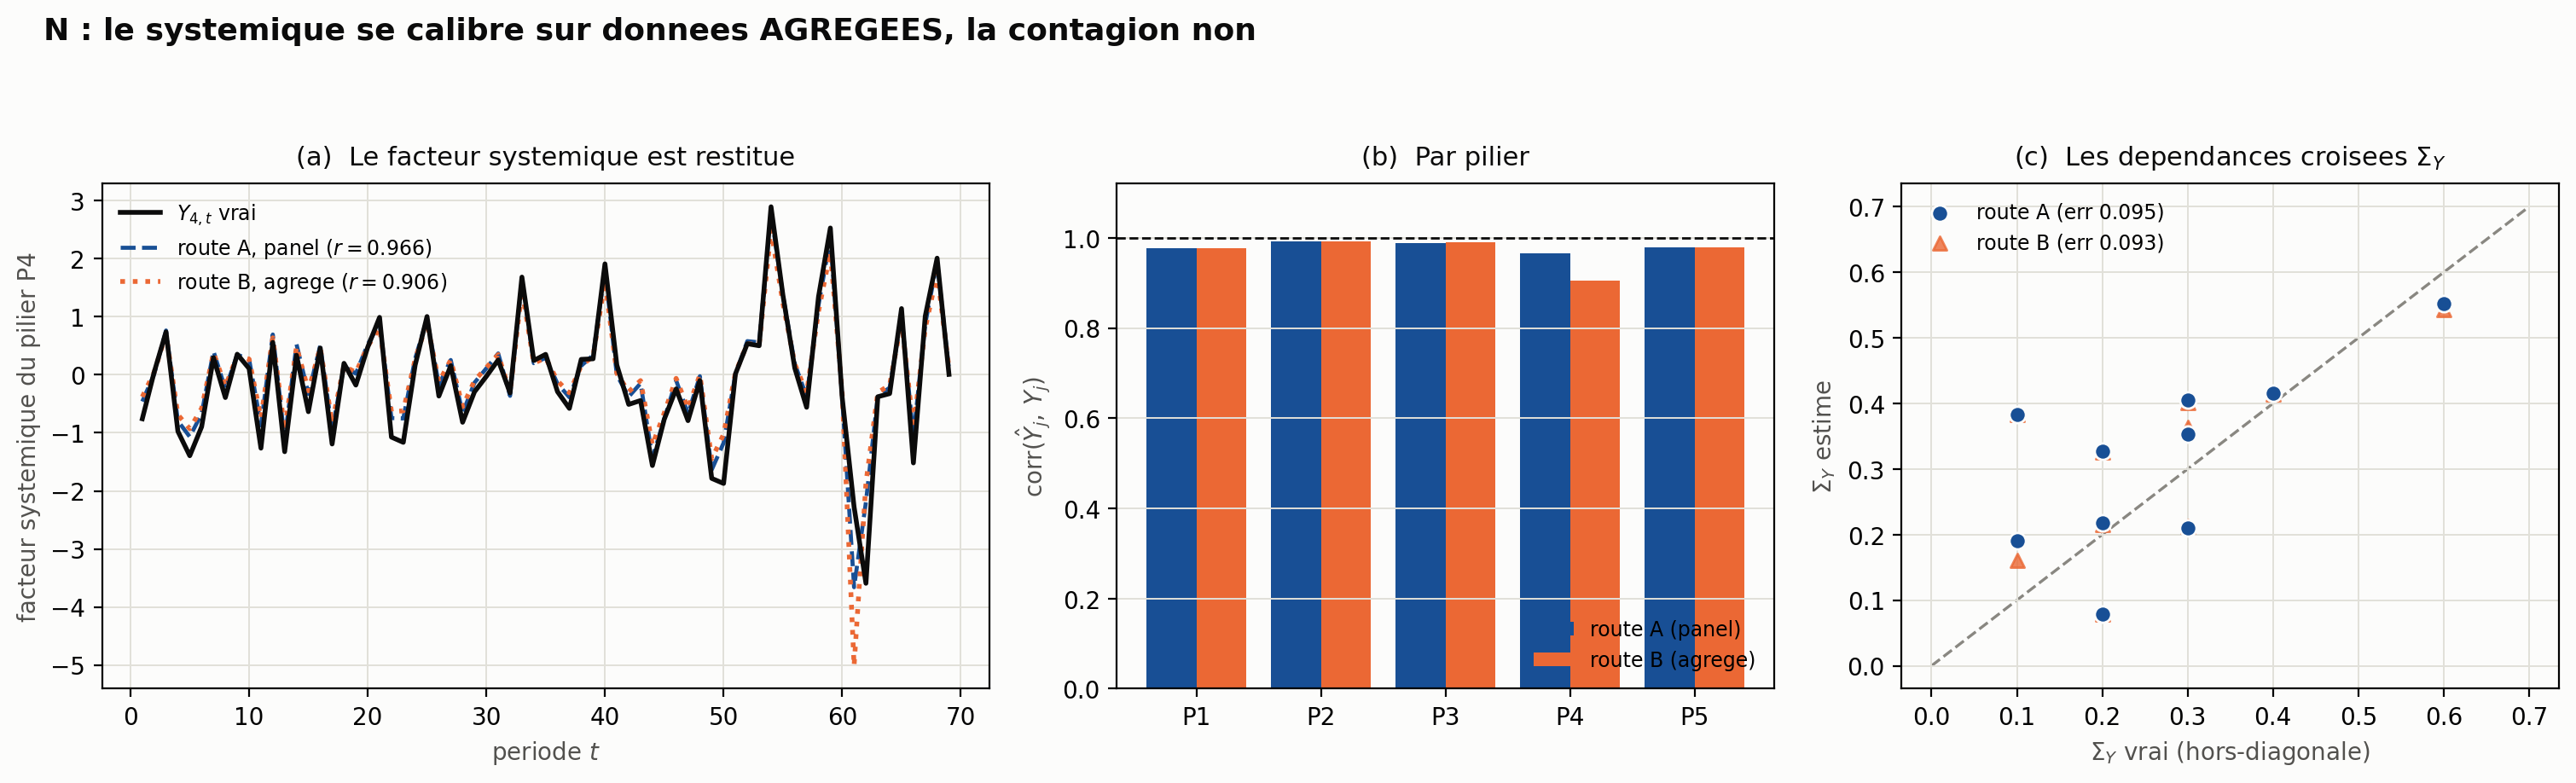
\includegraphics[width=\textwidth]{../figures/N_facteur_systemique.png}
\caption{Le facteur systémique par pilier est restitué par les deux routes. (a)~série
temporelle du pilier P4, celui de plus forte charge ; (b)~corrélation pilier par pilier ;
(c)~les dépendances croisées $\Sigma_Y$, estimées contre vraies.}
\end{figure}

\section{Ancienne méthode contre nouvelle méthode}

\begin{table}[h]
\centering
\small
\caption{Ce qui a changé.}
\begin{tabularx}{\textwidth}{>{\raggedright\arraybackslash}p{3.5cm} >{\raggedright\arraybackslash}X >{\raggedright\arraybackslash}X}
\toprule
\textbf{Objet} & \textbf{Ancienne méthode} & \textbf{Nouvelle méthode} \\
\midrule
Effets fixes de période
  & Mal indexés (\texttt{repeat}) : n'absorbaient rien. Le systémique polluait l'erreur.
  & Correctement indexés (\texttt{tile}) : ils absorbent le systémique \emph{et} le mesurent. \\
\addlinespace
Échelle du probit
  & Atténuée de $0{,}894$ sans qu'on le sache. Pente $0{,}92$.
  & Non atténuée. Pente $1{,}08$ : $W$ dans ses propres unités. \\
\addlinespace
Charges $s_j$
  & Non estimées. Postulées.
  & Estimées : écart-type temporel des effets fixes. \\
\addlinespace
Facteur $\Y_{j,t}$
  & Non estimé. Objet purement théorique.
  & Restitué à $\mathrm{corr} = 0{,}98$ (A) ou $0{,}97$ (B). \\
\addlinespace
Dépendances $\Sigma_Y$
  & Non estimées.
  & Corrélation des effets fixes ; erreur $\approx 0{,}09$. \\
\addlinespace
Donnée requise pour le systémique
  & (question non posée)
  & \textbf{Comptages agrégés} par pilier et par période. Aucun identifiant d'entité. \\
\addlinespace
Donnée requise pour $W$
  & Panel individuel horodaté
  & Panel individuel horodaté au mois \emph{(inchangé : introuvable, cf.~script \texttt{05})} \\
\bottomrule
\end{tabularx}
\end{table}

\section{Ce que cela change pour le mémoire}

\begin{cle}
\textbf{Le verrou est plus étroit qu'annoncé, et c'est un résultat positif.} Le chapitre de
faisabilité concluait que le modèle n'était pas calibrable sur les sources disponibles. Cette
conclusion vaut pour~$W$, et pour~$W$ seulement. La route~B n'utilise \textbf{aucun
identifiant d'entité} : uniquement des comptages agrégés par pilier et par période. Or c'est
précisément ce que publient déjà les registres DORA, l'ENISA et les CERT.
\end{cle}

\begin{center}
\small
\begin{tabular}{lll}
\toprule
\textbf{Objet du modèle} & \textbf{Donnée requise} & \textbf{Disponible ?} \\
\midrule
Contagion dirigée $W$          & panel individuel horodaté au mois & \textbf{non} \\
$\Y_j$, $s_j$, $\Sigma_Y$      & statistiques agrégées publiques   & \textbf{oui} \\
\bottomrule
\end{tabular}
\end{center}

\medskip
\noindent
Autrement dit : la \textbf{généralisation~A}, un facteur systémique par pilier avec ses
charges et ses dépendances croisées, ce qui est déjà une rupture nette avec le Vasicek à un
facteur, est calibrable \textbf{dès aujourd'hui}, sur données publiques. Seule la
\textbf{généralisation~B}, la contagion dirigée, attend sa donnée. Le chapitre négatif
devient un chapitre à deux régimes.

\section{Limites, dites franchement}

\begin{attention}
\textbf{Trois réserves qu'il ne faut pas laisser sous silence.}
\begin{enumerate}[leftmargin=1.6em,itemsep=2pt]
\item \textbf{Tout ceci est établi sur données simulées.} Le processus générateur est connu,
donc les deux routes sont validées contre une vérité que l'on possède. C'est une preuve de
correction de l'estimateur, \textbf{pas} une preuve que le modèle décrit le monde.
\item \textbf{La route~B suppose $W$ et base connues.} Elle extrait le systémique
\emph{conditionnellement} à la contagion. Comme $W$ n'est pas calibrable, il faudra en
pratique la balayer sur le gain admissible $g \in (0,1]$ et vérifier que $\hat{\Y}$ est stable.
Cette vérification n'est pas faite.
\item \textbf{$\Sigma_Y$ est le maillon faible.} L'erreur absolue moyenne de $0{,}09$ paraît
bonne, mais la corrélation entre les dix coefficients hors-diagonale vrais et estimés ne vaut
que $0{,}67$. On retrouve le \emph{niveau} des dépendances croisées, pas finement leur
\emph{structure}. Sur $T = 70$ périodes, c'est un problème d'échantillon, et il faut le dire.
Le pilier P4 en porte la trace : $\hat{s}_4 = 0{,}745$ contre $0{,}60$ par la route~B.
\end{enumerate}
\end{attention}

\section*{Reproductibilité}

\begin{center}
\small
\begin{tabular}{ll}
\toprule
\textbf{Script} & \textbf{Produit} \\
\midrule
\texttt{03\_calibration\_W.py} & figures K1, K2, K3 ; indexation corrigée \\
\texttt{06\_facteur\_systemique.py} & figure N ; routes A et B \\
\bottomrule
\end{tabular}
\end{center}

\medskip
\noindent
\small
Graine \texttt{20260710}. Dépendances : \texttt{numpy}, \texttt{scipy}, \texttt{statsmodels},
\texttt{matplotlib}. Référence : Pineau, É. et Zuñiga, F. (2023), pour la méthode d'extraction
de facteur par distance de Frobenius.

\end{document}
